\section{Overview}\seclabel{Overview}

In this section, we provide an informal overview of our approach using a simple example.

\begin{figure}
\centering
\begin{tabular}{ccc}
\begin{lstlisting}
int sign(int x) { 
  int sgn;
  if (x < 0)
    sgn = -1
  else 
    sgn = 1
 return sgn
}
(*@ \vspace{0.1in} @*)
\end{lstlisting}
&
&
\begin{lstlisting}
int sign'(int x) {
  int sgn;
  if (x < 0)
    sgn = -1
  else if (x==0)
    sgn = 0
  else 
    sgn = 1
 return sgn
}
\end{lstlisting}
\\
\end{tabular}
\caption{Two simple implementations of the \emph{sign} operation.}
\figlabel{SignExample}
\end{figure}


Consider the two simple example programs of~\figref{SignExample}, inspired by an example from~\cite{MauborgneRival07}. For these two programs, we would like to establish that the output of $sign$ and $sign'$ only differs in the case where $x=0$ and that the difference is $sgn = 1 \neq sgn' = 0$. A precise characterization of behavior is the following:

\vspace{0.1in}
{\footnotesize
\begin{tabular}{l|l|l}
$x.x'$ constraints  & $sgn$             & $sgn'$
\\ \hline
$x < 0$             & $sgn \mapsto -1$  & $sgn' \mapsto -1$
\\ \hline
$x = 0$             & $sgn \mapsto 1$  & $sgn' \mapsto 0$
\\ \hline
$x > 0$             & $sgn \mapsto 1$  & $sgn' \mapsto 1$
\end{tabular}
}

\para{Separate Analysis is Unsound}
As a first naive attempt to achieve such a description, one could try to analyze each version of the program separately and compare the (abstract) results. However, this is clearly unsound, as equivalence under abstraction does not entail concrete equivalence. For example, using a interval analysis~\cite{CousotHalbwachs78} would yield that in both programs the value of \scode{sgn} ranges in the same interval $[-1,1]$, missing the fact that $sign$ never returns the value $0$.

%Furthermore, this representation ignores how $x$ affects the value of $sgn$ thus we would have no means to differentiate correctly, by input (e.g. we will get the same result for the $-1 * sign$ function).

\para{Establishing Equivalence under Abstraction}
To establish equivalence under abstraction, we need to abstract \emph{relationships between the values of variables} in $sign$ and $sign'$. Specifically, we need to track the relationship between the values of \scode{sgn} in both versions. Tracking relationships between variables of two program versions requires a joint representation in which these relationships can be tracked.

\para{Correlating Program} As a first step, our goal is to construct a program in which we can track relationships between variables of $sign$ and $sign'$. One naive option would be to construct a program $P;P'$ by sequentially composing the two program versions (as in \cite{EnglerRamos11}). However, establishing equivalence between variables in such program requires an analysis to precisely track paths across $P$ so they can be later compared to the corresponding paths in $P'$. \figref{SignAnalysis1} informally illustrates the paths that have to be correlated through $sign;sign'$ to track the relationship between \scode{sgn} and \scode{sgn'}. To establish equivalence between \scode{sgn} and \scode{sgn'} an analysis must separately track paths in $sign$ that lead to different values of \scode{sgn} until it reaches a corresponding path in $sign'$ which produces an equivalent value for \scode{sgn'}.

Intuitively, establishing equivalence using the sequential composition $P;P'$ might require full path sensitivity, leading to an inherently non-scalable solution. Further, in the presence of loops and widening, applying widening separately to the loops of $P$ and to those of $P'$ may completely jeopardize any attempt to maintain relationships under abstraction.

To address these challenges, we construct a \emph{correlating program} $P \correlate P'$ where operations of $P$ and $P'$ are carefully interleaved to keep execution of both versions close to lock-step progress. \figref{SignCorrelating} shows the correlating program for the programs of~\figref{SignExample}. The programs were transformed to a guarded command language form to allow for interleaving. Using the correlating program, we can directly track the relationship between \scode{sgn} in $sign$ and its corresponding variable \scode{sgn'} in $sign'$. \secref{Correlating} provides more details on the construction of a correlating program.

\para{Correlating Abstract Domain}
To analyze a given correlating program, we introduce a \emph{correlating abstract domain} that tracks relationships between corresponding variables in $P$ and $P'$ by tracking relationship in the correlating program $P \correlate P'$. Unfortunately, any domain with convex constraints will still fail to capture the precise relationship between \scode{sgn} and \scode{sgn'}. For example, using the polyhedra abstract domain~\cite{CousotHalbwachs78}, the relationship between \scode{sgn} and \scode{sgn'} in the correlating program would be lost, leaving only the trivial $\langle 1 \geq sgn \geq -1, 1 \geq sgn' \geq -1 \rangle$ constraint. Although the result soundly reports a difference, we still know nothing of the difference between the programs.

An obvious, but prohibitively expensive, solution to the problem is to use disjunctive completion~\cite{TODO}, moving to a powerset domain in which every abstract state is a set of convex objects (e.g., set of polyhedra).
A state in such domain is a set of convex abstract representations (e.g., polyhedra~\cite{CousotHalbwachs78} or octagon~\cite{Mine2006}). For example, analyzing $sign \correlate sign'$ using a powerset domain would yield:

\vspace{0.1in}
\begin{tabular}{ccc}
\hspace{1cm} $\sigma_{\times}^1 = \{x = x' < 0, sgn = sgn' \mapsto -1\}$
\\
\hspace{1cm} $\sigma_{\times}^2 = \{x = x' = 0, sgn \mapsto 1, sgn' \mapsto -1\}$
\\
\hspace{1cm} $\sigma_{\times}^3 = \{x = x' > 0, sgn = sgn' \mapsto 1\}$
\\
\end{tabular}
\vspace{0.1in}

However, using such domain would significantly limit the applicability of the approach. The desirable solution is a partially disjunctive domain, in which only certain disjunctions are kept separate during the analysis, while others are merged. The challenge in our setting is in keeping the partition fine enough such that equivalence could be preserved, without reaching exponential blowup.

As the goal of work is to distinguish equivalent from differencing behaviors, using equivalence as criteria for merging paths is apt. The partitioning will abstract together paths that hold equivalence for the same set of variables, allowing for a maximum of $2^{|VC|}$ disjunctions in the abstract state, where $VC$ is the set of correlated variables. So far we have implicitly defined $VC$ as a correlation between $P,P'$ input and outputs, but our approach is in fact parameterized by this matching, allowing for any $P$ variable to be matched with any of $P'$ which has the potential to provide a more precise result (in the cost of scaling) or alternatively provide a more coarse, scalable result by allowing less variables or only certain equivalence classes of $2^{VC}$. A formal definition and discussion of $VC$ is found in \secref{ConcreteSem}.

For example partitioning the result of \figref{SignAnalysis1} according to our criteria would abstract behaviors $s_1$ and $s_3$ together, as they hold equivalence for $sgn$. The merge would abstract away data regarding $x$ and represent $sgn$ as the $[-1,1]$ interval, losing precision but gaining reduction in state size. This loss of precision is acceptable as it is complemented by the offending state $s_2$.

%Still, not much is gained from this partitioning, as it is performed at the final state, where we may have already reached an exponential amount of disjunctions.

\vspace{0.1in}
\begin{tabular}{ccc}
\hspace{1cm} $\sigma_{\times}^1 = \{x = x', sgn = sgn' \mapsto [-1,1]\}$
\\
\hspace{1cm} $\sigma_{\times}^2 = \{x' = 0, sgn \mapsto 1, sgn' \mapsto -1\}$
\\
\end{tabular}
\vspace{0.1in}

\begin{figure}
\centering
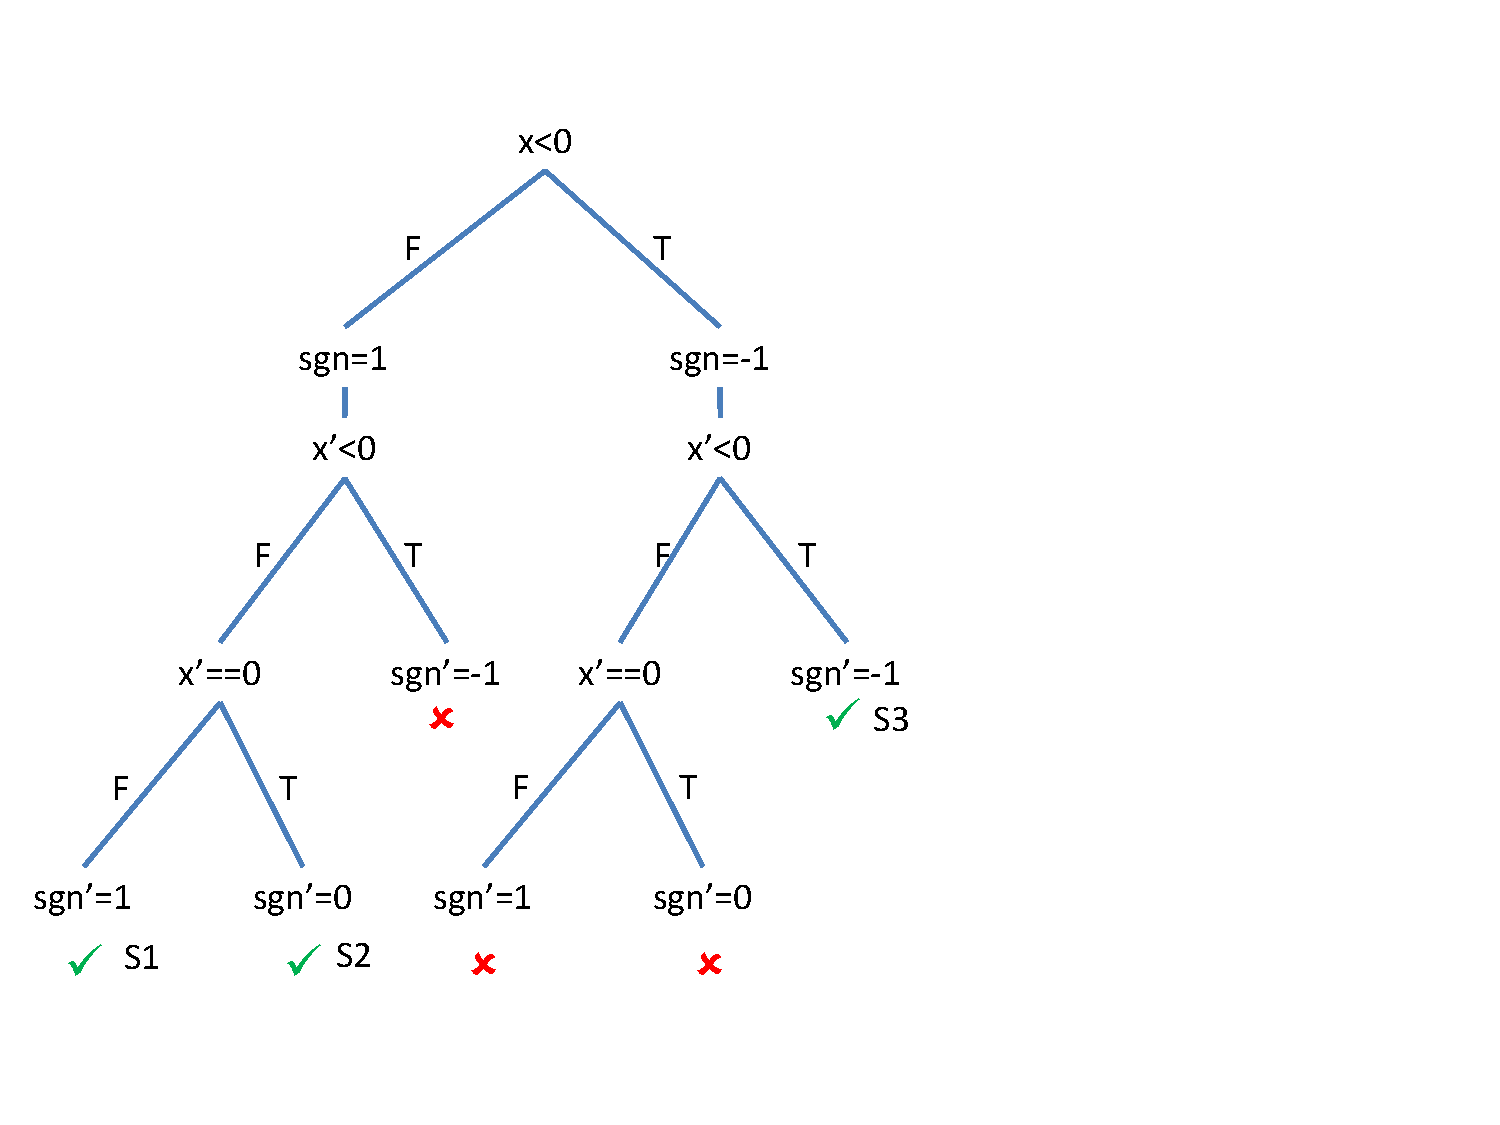
\includegraphics[scale=0.38,clip=true,trim = 75pt 25pt 5pt 20pt]{figures/sign-graph-joint}
\caption{Joint $sign;sign'$ analysis}\figlabel{SignAnalysis1}
\end{figure}



\begin{figure}
\centering
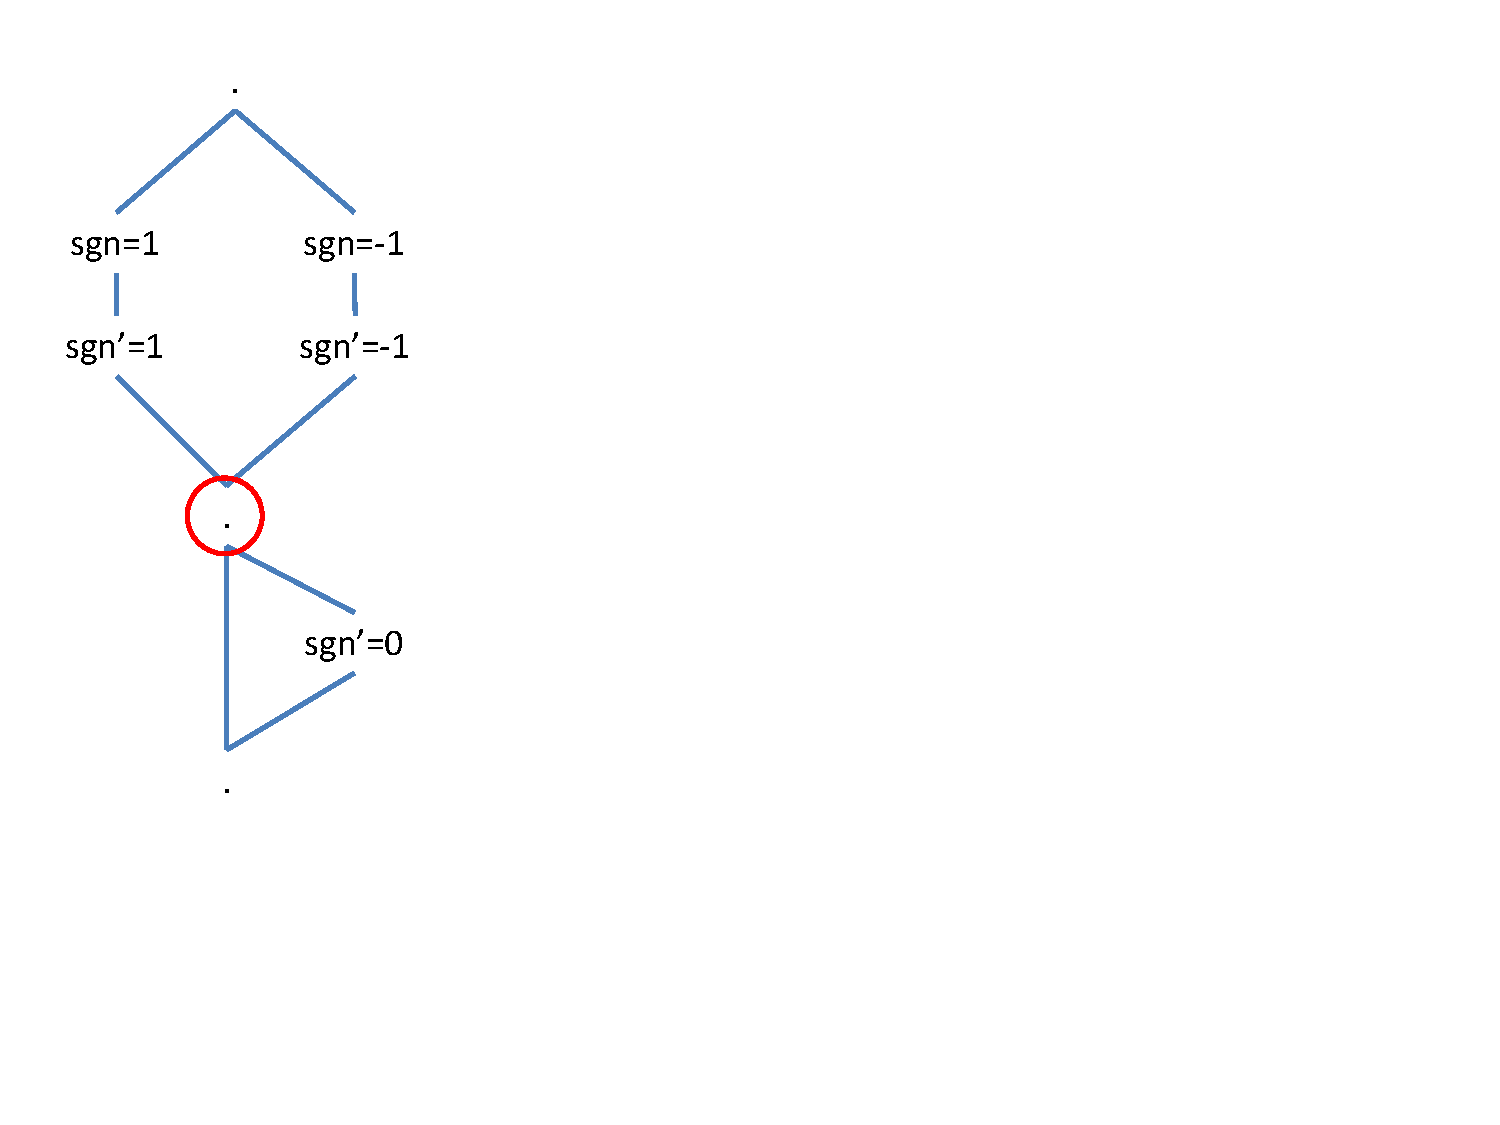
\includegraphics[scale=0.42,clip=true,trim = 0pt 150pt 450pt 150pt]{figures/sign-graph-correlated}
\caption{$sign \bowtie sign'$ analysis}\figlabel{SignAnalysis2}
\end{figure}

To gain a reduction of state size, we must perform partitioning dynamically during analysis. This cannot be achieved using a sequential composition $P;P'$. Looking at \figref{SignAnalysis1} we see that equivalence holds only at final states. Intuitively, this is because an operation in $P$ having to "wait" for its equivalent operation to occur in $P'$. To overcome this, our correlating program $P \bowtie P'$ interleaves $P$ and $P'$ commands in an optimized manner, and informs the analysis when programs have reached a point in which correlation can be established.  
\figref{SignAnalysis2} shows the analysis of $sign \bowtie sign'$ (shown in \figref{SignCorrelating}) where the correlating location is marked with a circle. The choice of \emph{correlation points} (denoted $CP$) is done during the construction of the correlating program. We describe the specifics of creating $P \bowtie P'$ in \secref{Correlating} and only briefly note that the interleaving is chosen according to a syntactic diff process over a guarded command language version of the programs.

\begin{figure}
\centering
\begin{lstlisting}
// Nimrod - please fill this 
\end{lstlisting}
\caption{Correlating program $sign \correlate sign'$.}
\figlabel{SignCorrelating}
\end{figure}


\para{Windening}
% bite the bullet and do widening.
Although we achieved a reduction in state size using partitioning, we have yet to account for programs with loops. Handling loops is where most previous approaches fall short~\cite{GodlinStrichman09, KawaguchiLahiriRebelo10, DwyerElbaumPerson08, EnglerRamos11}. To overcome this, we define a widening operator for our domain, based on the convex sub-domain widening operator. The main challenge here, as our state is a set of convex objects, is finding an optimal pairwise matching between objects for a precise widened result. Ideally, we would like to pair objects that adhere to the same ``looping path'' meaning we would like to match a path $\pi_i$'s abstraction with a path $\pi_{i+1}$ that results from taking another step in the loop. This requires encoding path information along with the sub-state abstraction. This information is acquired by keeping guard values explicitly, as they appear in our correlating program, inside the state. As guard values (true or false) reflect branch outcomes, they can be used to match sub-states that advanced on the loop by matching their guard values.

\begin{figure}
\centering
\begin{lstlisting}
int sum(int arr[], unsigned len) {
  int result = 0;
  for (unsigned i = 0; i < len; i++)
    result += arr[i];
 return result;
}
\end{lstlisting}
\caption{A simple looping program for array summation.}
\figlabel{LoopExample}
\end{figure}

We note that the correlating program is cruicial to maintaining equivalence over loops. To demonstrate this we perform the simple exercise of checking equivalence of a small looping program with itself. Consider the array summation program in \figref{LoopExample}. Equivalence for these two small programs cannot be established soundly by approached based on under approximation. To emphasize the importance of the correlating program, we will first show the result of an analysis of $sum;sum'$ which will be:
\\
\begin{tabular}{c}
\hspace{1cm} $\sigma_{\times}^1 = \{len = len' \leq 1, result = result' \mapsto 0\}$
\\
\hspace{1cm} $\sigma_{\times}^2 = \{len = len' > 1\}$
\end{tabular}
\\
\begin{figure}
\centering
\begin{lstlisting}
int sum(int arr[], unsigned len) {
  unsigned len' = len;
  int arr'[] = arr;
  int result = 0;
  int result' = 0;
  {
    unsigned i = 0;
    unsinged i' = 0;
l:  guard g = (i < len);
l': guard g' = (i' < len');
    if (g) result += arr[i];
    if (g') result' += arr'[i'];
    if (g) i++;
    if (g') i'++;
    if (g) goto l;
    if (g') goto l';
  }
}
\end{lstlisting}
\caption{$sum \bowtie sum$}
\figlabel{LoopExample}
\end{figure} 
This loss of equivalence occurred due to the inability precisely track the relationship of $result$ and $result'$ over $sum;sum'$. As we widened the first loop to converge, all paths passing through that loop were merges together, losing the ability to be "matched" with the second loop waiting further down the road. Performing the same analysis on $sum \bowtie sum'$ instead (seen in \figref{LoopCorrelatingExample}), allows maintaining equivalence, as the loops are interleaved correctly to allow establishing $result = result'$ as a loop invariant, surviving the widening process to prove equivalence at the end as the result would be:
\\
\begin{tabular}{c}
\hspace{2cm} $\sigma_{\times}^1 = \{result = result'\}$
\end{tabular}
\\
%The conceptual difference of these two analyses is depicted in \figref{SumWidening}.
%\begin{figure}
%\imagetop{
%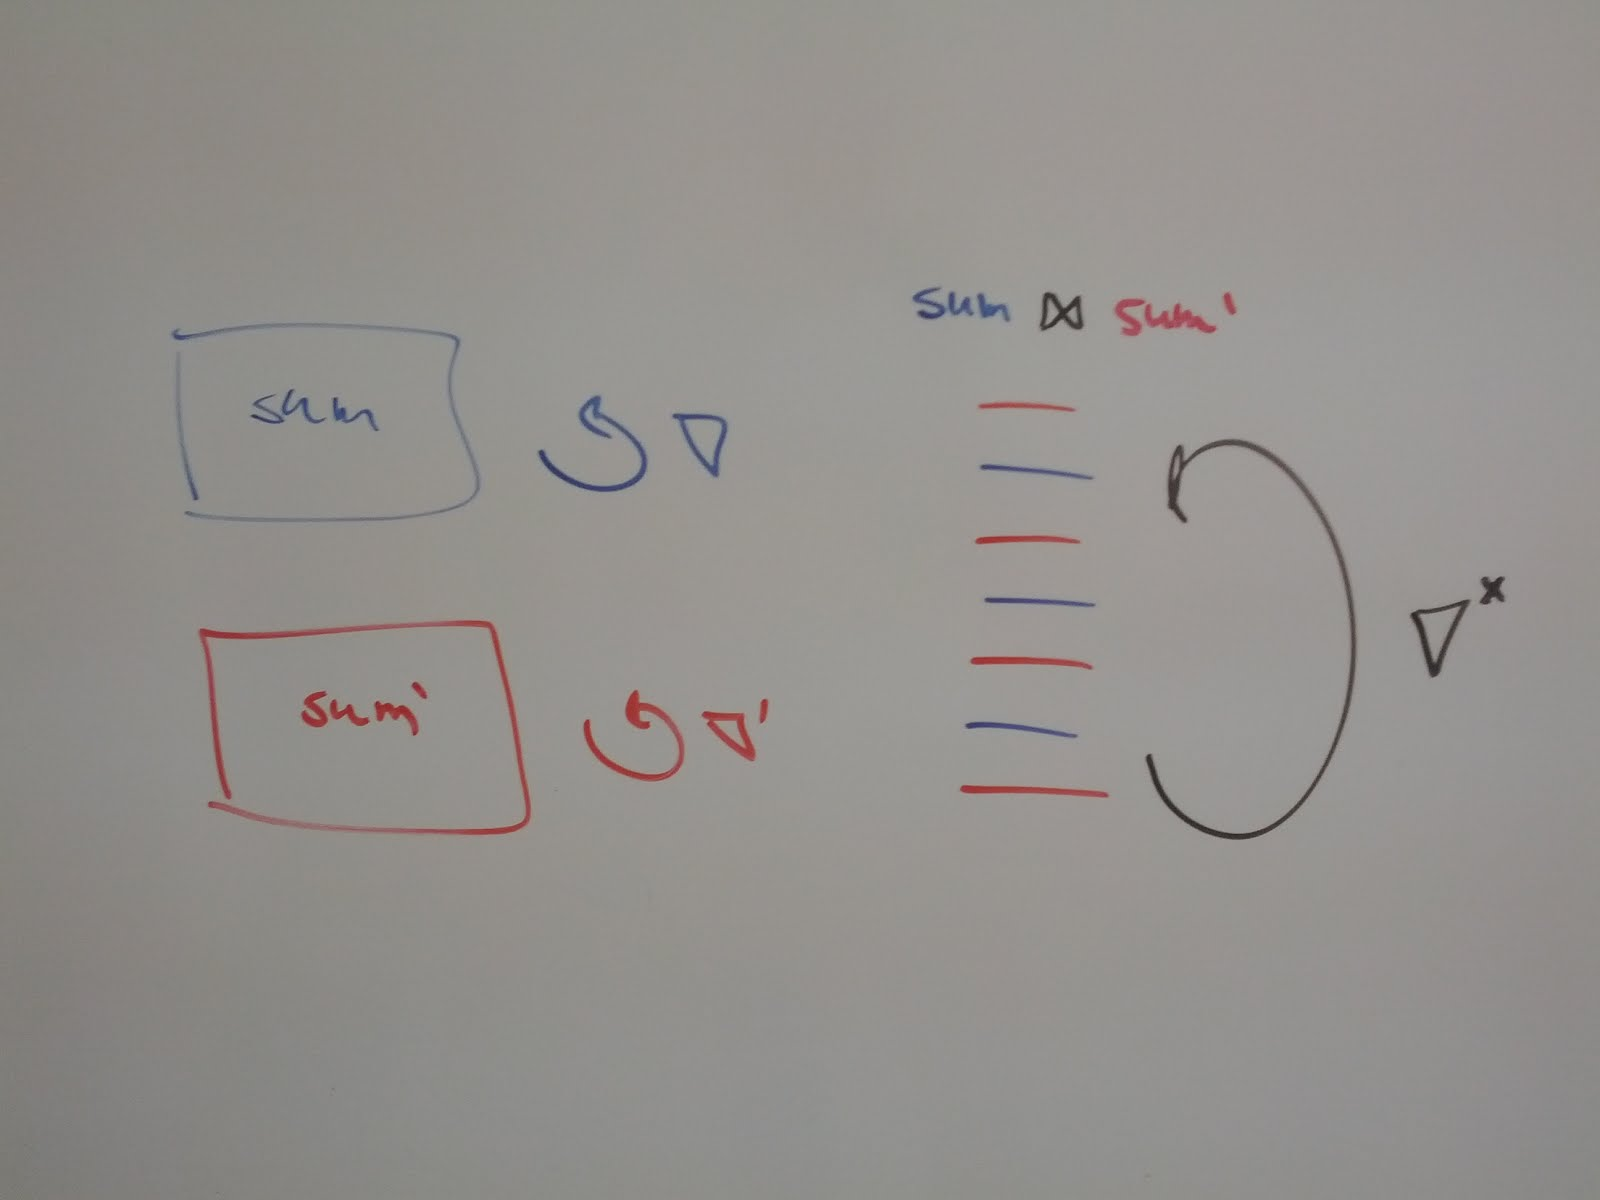
\includegraphics[scale=0.20,clip=true,trim = 150pt 250pt 200pt 200pt]{figures/sum-widening.jpg}
%}
%\caption{Widening $sum ; sum$ vs. $sum \bowtie sum$}\figlabel{SumWidening}
%\end{figure}

\paragraph{Definition of difference}
So far, we defined difference in programs as difference in output variable values at the program final state. Our work extends the notion of difference beyond that, allowing for several program locations to be identified as viable for differentiation (we name these locations \emph{differencing points} denoted $DP$). Other than the programs endpoints, we include every location which:
\begin{itemize}
\item Emits an output value (using a system function or through a global variable)
\item Accesses array
\end{itemize}
This means that procedures may now differ, even if they hold equivalence on the final state. Thus we define difference also as producing a different output value in mid-execution or accessing an array through a different index. This means that programs which differ in array access \emph{patterns} will now be flagged as different. This is a sound approach for difference, as this may include access to illegal bounds (an example for this can be seen in \figref{Md5sumExample}). We note that this definition of description cannot be achieved by instrumenting output or array access through temporary variables and deferring checking their equivalence to the end, as the amount of temporaries needed may be unbound. We therefore require procedures to agree on these locations, in case we wish to verify using the extended definition of difference. 